\section{Generátor zvuků}
Zvukový generátor je důležitou součástí \zkratka{LG} vesty. Zajišťuje generování zvuků, jejichž stěžejním cílem je informování hráčů o aktuálním dělení v aréně a také zlepšují výsledný prožitek ze hry.

\subsection{Požadavky na generátor}
Pro generátor je jedním z nejdůležitějších požadavků jeho paměť alespoň 1~\jedn{MB}. Možnost jej řídit pomocí \zkratka{UART}. Jednoduchá indikace přehrávání a možnost snížit odběr generátoru pomocí GPIO.

\subsection{Realizace generátoru}
\begin{figure}[H]
    \begin{center}
        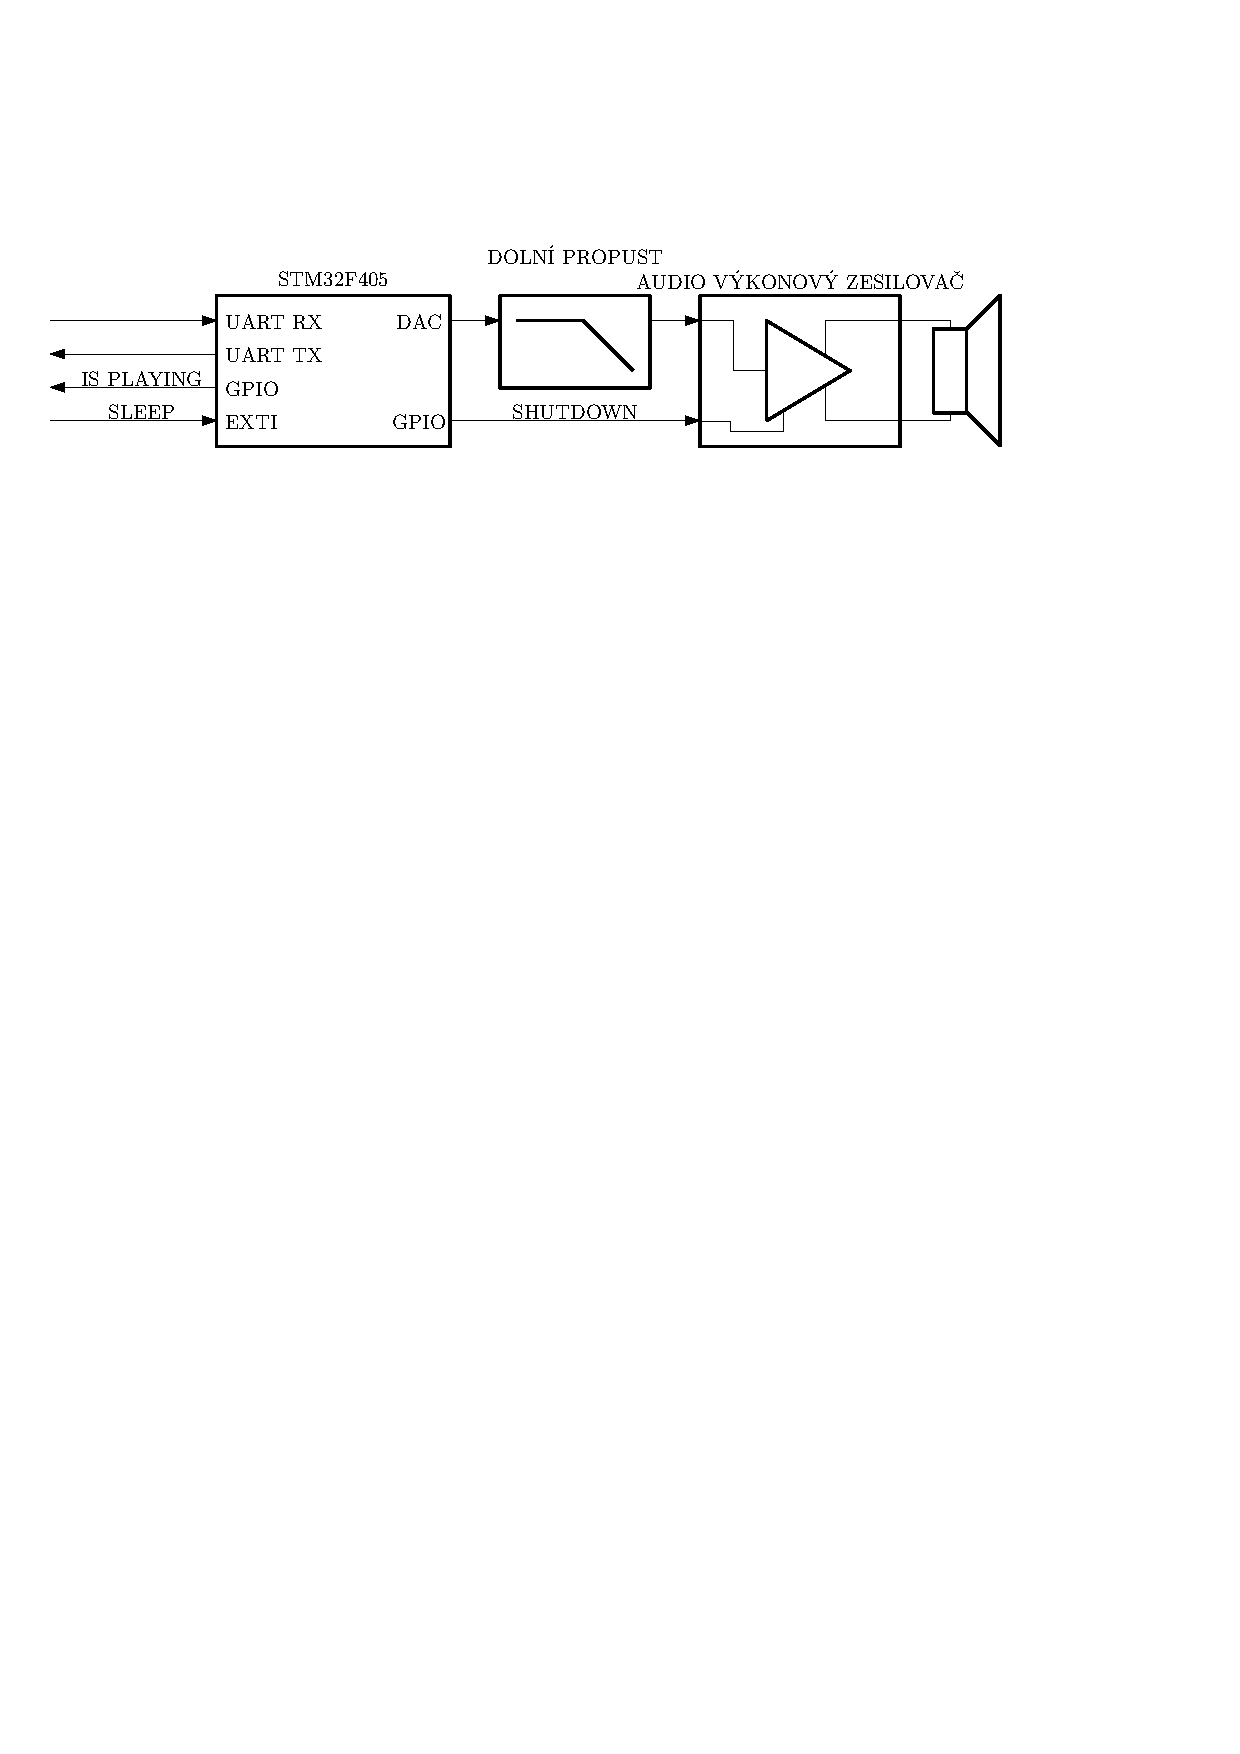
\includegraphics[width=\textwidth]{img/sound-system}
    \end{center}
    \caption{blokové znázornění zvukového generátoru}
\end{figure}

Generátor je založen na mikroprocesoru STM32F405, který je vybavený 1~\jedn{MB} paměti FLASH, která je využita, z velké části k uložení vzorků zvuků. Ve zbytku paměti je uložen firmware generátoru. Výše zmíněný mikroprocesor, také obsahuje mimo jiné 12~\jedn{b} DAC, až 32\jedn~{b} čítače / časovače, DMA, či
UART.

Zvuky jsou v paměti reprezentovány vzorky. Tedy polem kvantovaných hodnot snímaných v diskrétních časech, které popisují zvukové vlny.

Pokud chceme obnovit původní signál, je třeba tyto vzorky signálu ve stejných časech převádět pomocí DAC na napětí. K tomu je využita jednotka DMA a časovač. DMA je nakonfigurováno tak, aby přenášelo vzorky vybraného zvuku z paměti FLASH do DAC. Jednotka DAC je přitom spouštěna časovačem, který generuje spouštěcí signál stejnou frekvencí jako byla vzorkovací frekvence zvuků, tedy 16~\jedn{kHz}. Na výstupu mikroprocesoru tedy můžeme pozorovat napětí odpovídající hodnotám vzorků.

Následně je třeba signál obnovit pomocí rekonstrukčního (anti-aliasingového) filtru, tedy filtru typu dolní propust. Ten ze signálu odstraní nežádoucí spektrální složky, které vznikají skoky z hodnoty jednoho vzorku na vzorek druhý.

Poté je signál zesílen ve výkonovém integrovaném audio zesilovači LM4861 a přiveden do reproduktoru, kde dojde k jeho převodu na mechanické vlnění.
